%
%	Theorieteil
%

\pagebreak
\section{Data Exploration}

\onehalfspacing

\subsection{Data Layout}

The data consists of twelve datasets, one per year (3) and one per CNI (4).

After our data wrangling, all datasets now contain the following five blocks of metrics in a single row per observation:

\begin{itemize}
    \item Idle server memory and CPU consumption
    \item TCP Pod-to-Pod bandwidth, memory, and CPU consumption
    \item UDP Pod-to-Pod bandwidth, memory, and CPU consumption
    \item TCP Pod-to-Server bandwidth, memory, and CPU consumption
    \item UDP Pod-to-Server bandwidth, memory, and CPU consumption
\end{itemize}

For our data, Pod-to-Pod traffic refers to traffic between Pods in the same cluster, and Pod-to-Server traffic refers to traffic from a Pod to an outside application.

The individual field names are derived from each dataset's first row and are consistent across all sets.

\subsection{2020}

\subsubsection{Flannel}

The first data set we will look at is the 2020 data set for Flannel,
which we will read using R's built-in read.csv function.

\begin{Shaded}
\begin{Highlighting}[]
\NormalTok{main }\OtherTok{\textless{}{-}} \StringTok{"."}
\NormalTok{cni }\OtherTok{\textless{}{-}} \FunctionTok{read.csv}\NormalTok{(}\FunctionTok{here}\NormalTok{(main,}\StringTok{"data"}\NormalTok{,}\StringTok{"2020{-}flannel.csv"}\NormalTok{))}
\end{Highlighting}
\end{Shaded}

In the next step, we will have a look at the structure of our data and
visually inspect the measurements.

\begin{Shaded}
\begin{Highlighting}[]
\FunctionTok{str}\NormalTok{(cni)}
\end{Highlighting}
\end{Shaded}

\begin{verbatim}
'data.frame':   3095 obs. of  24 variables:
 $ smem  : num  593 596 590 591 588 ...
 $ scpu  : num  0.682 0.679 0.662 0.642 0.728 ...
 $ cmem  : num  588 595 591 587 592 ...
 $ ccpu  : num  0.572 0.601 0.54 0.517 0.579 ...
 $ tcpbw : num  9675 9757 9693 9689 9773 ...
 $ tcpsm : num  590 589 593 592 593 ...
 $ tcpsc : num  5.16 5.16 5.18 5.2 5.12 ...
 $ tcpcm : num  593 591 591 593 593 ...
 $ tcpcc : num  5.17 5.1 5.02 5.04 5.23 ...
 $ udpbw : num  9845 9842 9842 9841 9840 ...
 $ udpsm : num  591 590 592 594 589 ...
 $ udpsc : num  5.49 5.47 5.44 5.42 5.5 ...
 $ udpcm : num  608 611 608 613 614 ...
 $ udpcc : num  12.9 12.9 12.9 12.9 13 ...
 $ tcpebw: num  9831 9828 9827 9826 9838 ...
 $ tcpesm: num  589 596 591 590 589 ...
 $ tcpesc: num  4.92 5.07 5.08 5.03 5.14 ...
 $ tcpecm: num  595 601 595 595 593 ...
 $ tcpecc: num  5.47 5.55 5.46 5.52 5.29 ...
 $ udpebw: num  9823 9833 9818 9818 9833 ...
 $ udpesm: num  594 596 594 593 597 ...
 $ udpesc: num  5.25 5.3 5.34 5.41 5.23 ...
 $ udpecm: num  601 601 603 604 600 ...
 $ udpecc: num  12.6 12.7 12.7 12.7 12.6 ...
\end{verbatim}

The various values for memory consumption (MB), CPU usage (Percentage), and
bandwidth (MBit/s) look fine at first glance.

For further analysis, we will inspect the values a bit more
closely, starting with memory consumption. First, we'll look at the idle values and get:

\begin{Shaded}
\begin{Highlighting}[]
\FunctionTok{median}\NormalTok{(cni}\SpecialCharTok{\$}\NormalTok{smem)}
\end{Highlighting}
\end{Shaded}

\begin{verbatim}
[1] 592.8159
\end{verbatim}

\begin{Shaded}
\begin{Highlighting}[]
\FunctionTok{mean}\NormalTok{(cni}\SpecialCharTok{\$}\NormalTok{smem)}
\end{Highlighting}
\end{Shaded}

\begin{verbatim}
[1] 593.1625
\end{verbatim}

\begin{Shaded}
\begin{Highlighting}[]
\FunctionTok{min}\NormalTok{(cni}\SpecialCharTok{\$}\NormalTok{smem)}
\end{Highlighting}
\end{Shaded}

\begin{verbatim}
[1] 585
\end{verbatim}

\begin{Shaded}
\begin{Highlighting}[]
\FunctionTok{max}\NormalTok{(cni}\SpecialCharTok{\$}\NormalTok{smem)}
\end{Highlighting}
\end{Shaded}

\begin{verbatim}
[1] 606
\end{verbatim}

As the Median is more robust against outliers and works better with data that might be skewed, we'll focus on the median values going forward.\footnote{See \textit{Orn, A. (2023)}: Means and Medians: When To Use Which. \cite{meansMedians}}

Comparing the idle memory consumption with the other measurements for memory consumption (TCP and UDP, and Pod-to-Pod and Pod-to-Server), we get a fairly consistent picture:

\begin{Shaded}
\begin{Highlighting}[]
\FunctionTok{median}\NormalTok{(cni}\SpecialCharTok{\$}\NormalTok{tcpsm)}
\end{Highlighting}
\end{Shaded}

\begin{verbatim}
[1] 591.2724
\end{verbatim}

\begin{Shaded}
\begin{Highlighting}[]
\FunctionTok{median}\NormalTok{(cni}\SpecialCharTok{\$}\NormalTok{udpsm)}
\end{Highlighting}
\end{Shaded}

\begin{verbatim}
[1] 591.5915
\end{verbatim}

\begin{Shaded}
\begin{Highlighting}[]
\FunctionTok{median}\NormalTok{(cni}\SpecialCharTok{\$}\NormalTok{tcpesm)}
\end{Highlighting}
\end{Shaded}

\begin{verbatim}
[1] 590.1462
\end{verbatim}

\begin{Shaded}
\begin{Highlighting}[]
\FunctionTok{median}\NormalTok{(cni}\SpecialCharTok{\$}\NormalTok{udpesm)}
\end{Highlighting}
\end{Shaded}

\begin{verbatim}
[1] 594.3655
\end{verbatim}

Next, we will check CPU consumption, starting again with idle values:

\begin{Shaded}
\begin{Highlighting}[]
\FunctionTok{median}\NormalTok{(cni}\SpecialCharTok{\$}\NormalTok{scpu)}
\end{Highlighting}
\end{Shaded}

\begin{verbatim}
[1] 0.6546849
\end{verbatim}

\begin{Shaded}
\begin{Highlighting}[]
\FunctionTok{mean}\NormalTok{(cni}\SpecialCharTok{\$}\NormalTok{scpu)}
\end{Highlighting}
\end{Shaded}

\begin{verbatim}
[1] 0.6695833
\end{verbatim}

\begin{Shaded}
\begin{Highlighting}[]
\FunctionTok{min}\NormalTok{(cni}\SpecialCharTok{\$}\NormalTok{scpu)}
\end{Highlighting}
\end{Shaded}

\begin{verbatim}
[1] 0.6
\end{verbatim}

\begin{Shaded}
\begin{Highlighting}[]
\FunctionTok{max}\NormalTok{(cni}\SpecialCharTok{\$}\NormalTok{scpu)}
\end{Highlighting}
\end{Shaded}

\begin{verbatim}
[1] 0.82
\end{verbatim}

When we validate this with the other measurements for CPU consumption, we get again fairly consistent values across the measurements but a clear differentiation
to the idle values:

\begin{Shaded}
\begin{Highlighting}[]
\FunctionTok{median}\NormalTok{(cni}\SpecialCharTok{\$}\NormalTok{tcpsc)}
\end{Highlighting}
\end{Shaded}

\begin{verbatim}
[1] 5.162688
\end{verbatim}

\begin{Shaded}
\begin{Highlighting}[]
\FunctionTok{median}\NormalTok{(cni}\SpecialCharTok{\$}\NormalTok{udpsc)}
\end{Highlighting}
\end{Shaded}

\begin{verbatim}
[1] 5.483832
\end{verbatim}

\begin{Shaded}
\begin{Highlighting}[]
\FunctionTok{median}\NormalTok{(cni}\SpecialCharTok{\$}\NormalTok{tcpesc)}
\end{Highlighting}
\end{Shaded}

\begin{verbatim}
[1] 5.055657
\end{verbatim}

\begin{Shaded}
\begin{Highlighting}[]
\FunctionTok{median}\NormalTok{(cni}\SpecialCharTok{\$}\NormalTok{udpesc)}
\end{Highlighting}
\end{Shaded}

\begin{verbatim}
[1] 5.30168
\end{verbatim}

Idle CPU consumption does not seem to be a good overall performance indicator

The final data point we want to look at is bandwidth, the core
performance metric for a network:\footnote{See \textit{Solarwinds (2024)}: What are Network Performance Metrics? \cite{networkPerformance}}

\begin{Shaded}
\begin{Highlighting}[]
\FunctionTok{median}\NormalTok{(cni}\SpecialCharTok{\$}\NormalTok{tcpbw)}
\end{Highlighting}
\end{Shaded}

\begin{verbatim}
[1] 9705.809
\end{verbatim}

\begin{Shaded}
\begin{Highlighting}[]
\FunctionTok{median}\NormalTok{(cni}\SpecialCharTok{\$}\NormalTok{udpbw)}
\end{Highlighting}
\end{Shaded}

\begin{verbatim}
[1] 9843.559
\end{verbatim}

\begin{Shaded}
\begin{Highlighting}[]
\FunctionTok{median}\NormalTok{(cni}\SpecialCharTok{\$}\NormalTok{tcpebw)}
\end{Highlighting}
\end{Shaded}

\begin{verbatim}
[1] 9828.35
\end{verbatim}

\begin{Shaded}
\begin{Highlighting}[]
\FunctionTok{median}\NormalTok{(cni}\SpecialCharTok{\$}\NormalTok{udpebw)}
\end{Highlighting}
\end{Shaded}

\begin{verbatim}
[1] 9822.046
\end{verbatim}

With the majority of the internet traffic being TCP, we will focus on
the measurements for TCP for analysis and comparison.\footnote{See \textit{Quian, L. (2012)}: A flow-based performance analysis of TCP and TCP applications. \cite{tcpTraffic}}

We visualize both the TCP Pod-to-Pod and Pod-to-Server traffic bandwidth using histograms:

\begin{Shaded}
\begin{Highlighting}[]
\FunctionTok{gf\_histogram}\NormalTok{(}\SpecialCharTok{\textasciitilde{}}\NormalTok{tcpbw, }\AttributeTok{data =}\NormalTok{ cni")} 
\end{Highlighting}
\end{Shaded}

\begin{figure}[H]
\centering
\caption {FLannel Pod-to-Pod Bandwidth}
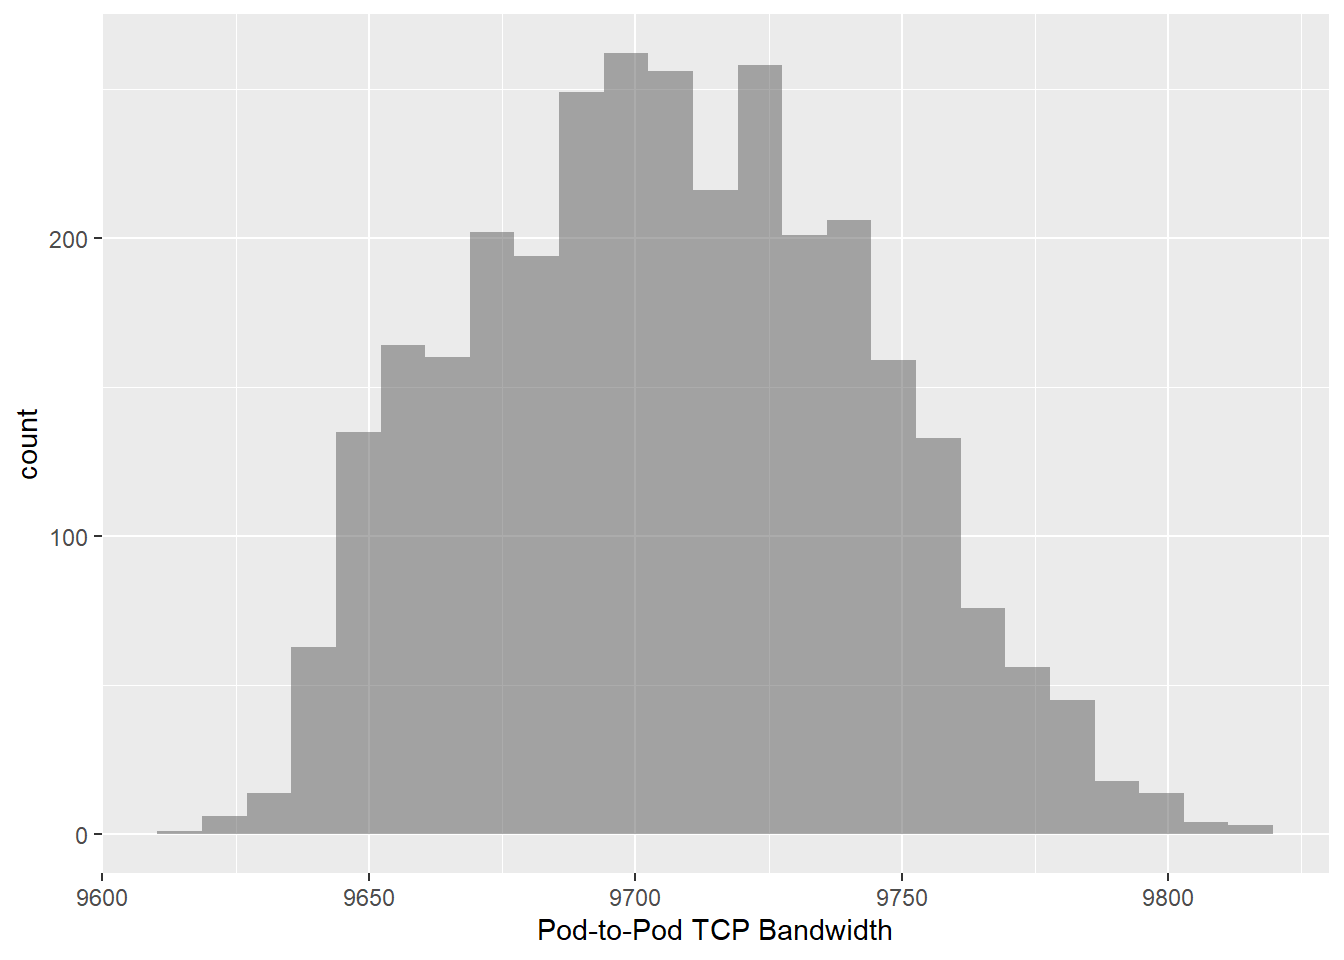
\includegraphics[width=\linewidth]{images/unnamed-chunk-8-1.png}
\label{fig:flannel-8-1}
\end{figure}

\begin{Shaded}
\begin{Highlighting}[]
\FunctionTok{gf\_histogram}\NormalTok{(}\SpecialCharTok{\textasciitilde{}}\NormalTok{tcpebw, }\AttributeTok{data =}\NormalTok{ cni")} 
\end{Highlighting}
\end{Shaded}

\begin{figure}[H]
\centering
\caption {FLannel Pod-to-Server Bandwidth}
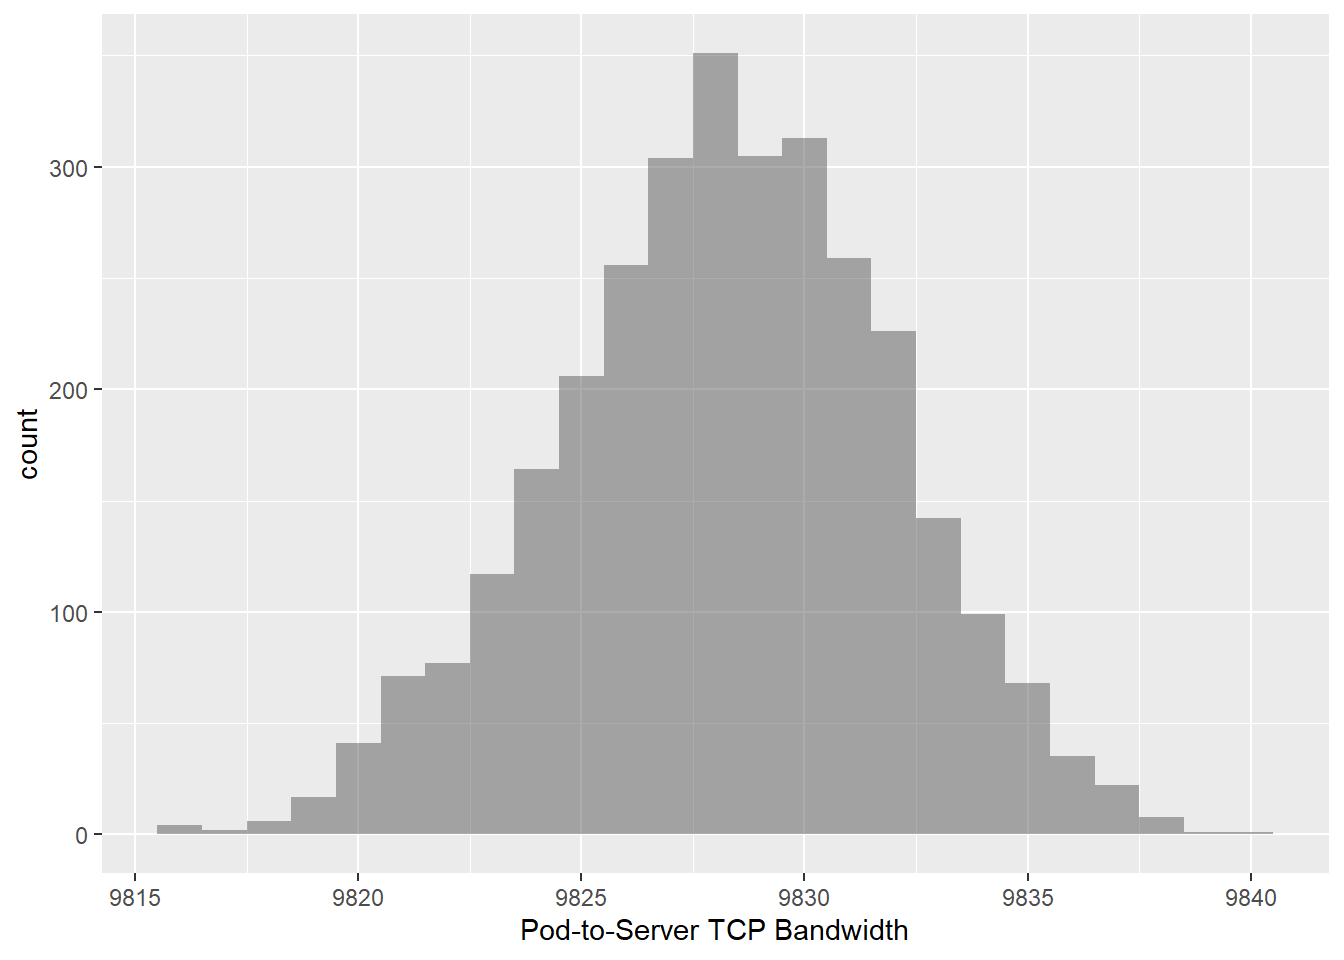
\includegraphics[width=\linewidth]{images/unnamed-chunk-9-1.png}
\label{fig:flannel-9-1}
\end{figure}

The data distribution supports our choice to use the median values as key indicators for TCP bandwidth.

Following the results of a scientific coin toss,\footnote{See \textit{Kim, S.E. (2024)}: Scientists Destroy Illusion That Coin Toss Flips Are 50–50. \cite{coinToss}} we will use the TCP Pod-to Server values for CPU usage and memory consumption for further analysis.

From the 2020 Flannel dataset, we will thus use the following values:

\begin{Shaded}
\begin{Highlighting}[]
\FunctionTok{median}\NormalTok{(cni}\SpecialCharTok{\$}\NormalTok{tcpesm)}
\end{Highlighting}
\end{Shaded}

\begin{verbatim}
[1] 590.1462
\end{verbatim}

\begin{Shaded}
\begin{Highlighting}[]
\FunctionTok{median}\NormalTok{(cni}\SpecialCharTok{\$}\NormalTok{tcpesc)}
\end{Highlighting}
\end{Shaded}

\begin{verbatim}
[1] 5.055657
\end{verbatim}

\begin{Shaded}
\begin{Highlighting}[]
\FunctionTok{median}\NormalTok{(cni}\SpecialCharTok{\$}\NormalTok{tcpbw)}
\end{Highlighting}
\end{Shaded}

\begin{verbatim}
[1] 9705.809
\end{verbatim}

\begin{Shaded}
\begin{Highlighting}[]
\FunctionTok{median}\NormalTok{(cni}\SpecialCharTok{\$}\NormalTok{tcpebw)}
\end{Highlighting}
\end{Shaded}

\begin{verbatim}
[1] 9828.35
\end{verbatim}

\subsubsection{Calico}

We will now read the 2020 data set for Calico.

\begin{Shaded}
\begin{Highlighting}[]
\NormalTok{main }\OtherTok{\textless{}{-}} \StringTok{"."}
\NormalTok{cni }\OtherTok{\textless{}{-}} \FunctionTok{read.csv}\NormalTok{(}\FunctionTok{here}\NormalTok{(main,}\StringTok{"data"}\NormalTok{,}\StringTok{"2020{-}calico.csv"}\NormalTok{))}
\end{Highlighting}
\end{Shaded}

In the next step, we will examine the structure of our data and visually
inspect the measurements.

\begin{Shaded}
\begin{Highlighting}[]
\FunctionTok{str}\NormalTok{(cni)}
\end{Highlighting}
\end{Shaded}

\begin{verbatim}
'data.frame':   3091 obs. of  24 variables:
 $ smem  : num  667 665 666 669 665 ...
 $ scpu  : num  1.64 1.64 1.62 1.64 1.63 ...
 $ cmem  : num  666 666 666 653 666 ...
 $ ccpu  : num  1.27 1.27 1.31 1.3 1.29 ...
 $ tcpbw : num  8879 8885 8884 8882 8884 ...
 $ tcpsm : num  660 664 662 664 660 ...
 ...
\end{verbatim}

Then, we'll extract the key metrics for further analysis:

\begin{Shaded}
\begin{Highlighting}[]
\FunctionTok{median}\NormalTok{(cni}\SpecialCharTok{\$}\NormalTok{tcpesm)}
\end{Highlighting}
\end{Shaded}

\begin{verbatim}
[1] 659.3846
\end{verbatim}

\begin{Shaded}
\begin{Highlighting}[]
\FunctionTok{median}\NormalTok{(cni}\SpecialCharTok{\$}\NormalTok{tcpesc)}
\end{Highlighting}
\end{Shaded}

\begin{verbatim}
[1] 6.44727
\end{verbatim}

\begin{Shaded}
\begin{Highlighting}[]
\FunctionTok{median}\NormalTok{(cni}\SpecialCharTok{\$}\NormalTok{tcpbw)}
\end{Highlighting}
\end{Shaded}

\begin{verbatim}
[1] 8882.457
\end{verbatim}

\begin{Shaded}
\begin{Highlighting}[]
\FunctionTok{median}\NormalTok{(cni}\SpecialCharTok{\$}\NormalTok{tcpebw)}
\end{Highlighting}
\end{Shaded}

\begin{verbatim}
[1] 8675.868
\end{verbatim}

\subsubsection{Canal}

We will now read the 2020 data set for Canal.

\begin{Shaded}
\begin{Highlighting}[]
\NormalTok{main }\OtherTok{\textless{}{-}} \StringTok{"."}
\NormalTok{cni }\OtherTok{\textless{}{-}} \FunctionTok{read.csv}\NormalTok{(}\FunctionTok{here}\NormalTok{(main,}\StringTok{"data"}\NormalTok{,}\StringTok{"2020{-}canal.csv"}\NormalTok{))}
\end{Highlighting}
\end{Shaded}

In the next step, we will examine the structure of our data and visually
inspect the measurements.

\begin{Shaded}
\begin{Highlighting}[]
\FunctionTok{str}\NormalTok{(cni)}
\end{Highlighting}
\end{Shaded}

\begin{verbatim}
'data.frame':   3076 obs. of  24 variables:
 $ smem  : num  662 659 663 663 663 ...
 $ scpu  : num  1.43 1.56 1.49 1.47 1.43 ...
 $ cmem  : num  663 663 660 666 659 ...
 $ ccpu  : num  1.97 2.01 1.98 1.99 1.96 ...
 $ tcpbw : num  8490 8586 8635 8647 8648 ...
 $ tcpsm : num  659 656 655 657 657 ...
 ...
\end{verbatim}

Then, we'll extract the key metrics for further analysis:

\begin{Shaded}
\begin{Highlighting}[]
\FunctionTok{median}\NormalTok{(cni}\SpecialCharTok{\$}\NormalTok{tcpesm)}
\end{Highlighting}
\end{Shaded}

\begin{verbatim}
[1] 655.4456
\end{verbatim}

\begin{Shaded}
\begin{Highlighting}[]
\FunctionTok{median}\NormalTok{(cni}\SpecialCharTok{\$}\NormalTok{tcpesc)}
\end{Highlighting}
\end{Shaded}

\begin{verbatim}
[1] 6.697056
\end{verbatim}

\begin{Shaded}
\begin{Highlighting}[]
\FunctionTok{median}\NormalTok{(cni}\SpecialCharTok{\$}\NormalTok{tcpbw)}
\end{Highlighting}
\end{Shaded}

\begin{verbatim}
[1] 8634.413
\end{verbatim}

\begin{Shaded}
\begin{Highlighting}[]
\FunctionTok{median}\NormalTok{(cni}\SpecialCharTok{\$}\NormalTok{tcpebw)}
\end{Highlighting}
\end{Shaded}

\begin{verbatim}
[1] 8576.709
\end{verbatim}

\subsubsection{Cilium}

We will now read the 2020 data set for Cilium.

\begin{Shaded}
\begin{Highlighting}[]
\NormalTok{main }\OtherTok{\textless{}{-}} \StringTok{"."}
\NormalTok{cni }\OtherTok{\textless{}{-}} \FunctionTok{read.csv}\NormalTok{(}\FunctionTok{here}\NormalTok{(main,}\StringTok{"data"}\NormalTok{,}\StringTok{"2020{-}cilium.csv"}\NormalTok{))}
\end{Highlighting}
\end{Shaded}

In the next step, we will examine the structure of our data and visually
inspect the measurements.

\begin{Shaded}
\begin{Highlighting}[]
\FunctionTok{str}\NormalTok{(cni)}
\end{Highlighting}
\end{Shaded}

\begin{verbatim}
'data.frame':   3082 obs. of  24 variables:
 $ smem  : num  859 867 863 857 863 ...
 $ scpu  : num  3.95 3.68 2.63 3.32 3.53 ...
 $ cmem  : num  867 872 871 868 864 ...
 $ ccpu  : num  1.78 1.74 1.69 1.73 1.76 ...
 $ tcpbw : num  9445 9547 9467 9449 9466 ...
 $ tcpsm : num  861 867 864 864 864 ...
 ...
\end{verbatim}

Then, we'll extract the key metrics for further analysis:

\begin{Shaded}
\begin{Highlighting}[]
\FunctionTok{median}\NormalTok{(cni}\SpecialCharTok{\$}\NormalTok{tcpesm)}
\end{Highlighting}
\end{Shaded}

\begin{verbatim}
[1] 866.5502
\end{verbatim}

\begin{Shaded}
\begin{Highlighting}[]
\FunctionTok{median}\NormalTok{(cni}\SpecialCharTok{\$}\NormalTok{tcpesc)}
\end{Highlighting}
\end{Shaded}

\begin{verbatim}
[1] 13.2222
\end{verbatim}

\begin{Shaded}
\begin{Highlighting}[]
\FunctionTok{median}\NormalTok{(cni}\SpecialCharTok{\$}\NormalTok{tcpbw)}
\end{Highlighting}
\end{Shaded}

\begin{verbatim}
[1] 9475.213
\end{verbatim}

\begin{Shaded}
\begin{Highlighting}[]
\FunctionTok{median}\NormalTok{(cni}\SpecialCharTok{\$}\NormalTok{tcpebw)}
\end{Highlighting}
\end{Shaded}

\begin{verbatim}
[1] 9673.348
\end{verbatim}

\subsection{2021}

\subsubsection{Flannel}

We will now read the 2021 data set for Flannel.

\begin{Shaded}
\begin{Highlighting}[]
\NormalTok{main }\OtherTok{\textless{}{-}} \StringTok{"."}
\NormalTok{cni }\OtherTok{\textless{}{-}} \FunctionTok{read.csv}\NormalTok{(}\FunctionTok{here}\NormalTok{(main,}\StringTok{"data"}\NormalTok{,}\StringTok{"2021{-}flannel.csv"}\NormalTok{))}
\end{Highlighting}
\end{Shaded}

In the next step, we will examine the structure of our data and visually
inspect the measurements.

\begin{Shaded}
\begin{Highlighting}[]
\FunctionTok{str}\NormalTok{(cni)}
\end{Highlighting}
\end{Shaded}

\begin{verbatim}
'data.frame':   3112 obs. of  24 variables:
 $ smem  : num  591 596 599 593 599 ...
 $ scpu  : num  0.67 0.665 0.699 0.654 0.699 ...
 $ cmem  : num  596 592 591 589 580 ...
 $ ccpu  : num  0.539 0.502 0.546 0.554 0.55 ...
 $ tcpbw : num  9657 9737 9680 9755 9689 ...
 ...
\end{verbatim}

Then, we'll extract the key metrics for further analysis:

\begin{Shaded}
\begin{Highlighting}[]
\FunctionTok{median}\NormalTok{(cni}\SpecialCharTok{\$}\NormalTok{tcpesm)}
\end{Highlighting}
\end{Shaded}

\begin{verbatim}
[1] 590.5901
\end{verbatim}

\begin{Shaded}
\begin{Highlighting}[]
\FunctionTok{median}\NormalTok{(cni}\SpecialCharTok{\$}\NormalTok{tcpesc)}
\end{Highlighting}
\end{Shaded}

\begin{verbatim}
[1] 5.015945
\end{verbatim}

\begin{Shaded}
\begin{Highlighting}[]
\FunctionTok{median}\NormalTok{(cni}\SpecialCharTok{\$}\NormalTok{tcpbw)}
\end{Highlighting}
\end{Shaded}

\begin{verbatim}
[1] 9695.797
\end{verbatim}

\begin{Shaded}
\begin{Highlighting}[]
\FunctionTok{median}\NormalTok{(cni}\SpecialCharTok{\$}\NormalTok{tcpebw)}
\end{Highlighting}
\end{Shaded}

\begin{verbatim}
[1] 9825.204
\end{verbatim}

The difference between the measurements in the 2020 and 2021 data sets is not that big; the data was taken only a couple of months apart, and the CNI versions were relatively close to each other.

\subsubsection{Calico}

We will now read the 2021 data set for Calico.

\begin{Shaded}
\begin{Highlighting}[]
\NormalTok{main }\OtherTok{\textless{}{-}} \StringTok{"."}
\NormalTok{cni }\OtherTok{\textless{}{-}} \FunctionTok{read.csv}\NormalTok{(}\FunctionTok{here}\NormalTok{(main,}\StringTok{"data"}\NormalTok{,}\StringTok{"2021{-}calico.csv"}\NormalTok{))}
\end{Highlighting}
\end{Shaded}

In the next step, we will examine the structure of our data and visually
inspect the measurements.

\begin{Shaded}
\begin{Highlighting}[]
\FunctionTok{str}\NormalTok{(cni)}
\end{Highlighting}
\end{Shaded}

\begin{verbatim}
'data.frame':   3103 obs. of  24 variables:
 $ smem  : num  663 669 663 665 667 ...
 $ scpu  : num  1.56 1.56 1.64 1.6 1.61 ...
 $ cmem  : num  666 664 665 669 667 ...
 $ ccpu  : num  1.25 1.24 1.25 1.27 1.24 ...
 $ tcpbw : num  8868 8875 8873 8867 8880 ...
 $ tcpsm : num  664 665 663 659 663 ...
 ...
\end{verbatim}

Then, we'll extract the key metrics for further analysis:

\begin{Shaded}
\begin{Highlighting}[]
\FunctionTok{median}\NormalTok{(cni}\SpecialCharTok{\$}\NormalTok{tcpesm)}
\end{Highlighting}
\end{Shaded}

\begin{verbatim}
[1] 661.9909
\end{verbatim}

\begin{Shaded}
\begin{Highlighting}[]
\FunctionTok{median}\NormalTok{(cni}\SpecialCharTok{\$}\NormalTok{tcpesc)}
\end{Highlighting}
\end{Shaded}

\begin{verbatim}
[1] 6.366529
\end{verbatim}

\begin{Shaded}
\begin{Highlighting}[]
\FunctionTok{median}\NormalTok{(cni}\SpecialCharTok{\$}\NormalTok{tcpbw)}
\end{Highlighting}
\end{Shaded}

\begin{verbatim}
[1] 8876.478
\end{verbatim}

\begin{Shaded}
\begin{Highlighting}[]
\FunctionTok{median}\NormalTok{(cni}\SpecialCharTok{\$}\NormalTok{tcpebw)}
\end{Highlighting}
\end{Shaded}

\begin{verbatim}
[1] 8763.889
\end{verbatim}

\subsubsection{Canal}

We will now read the 2021 data set for Canal.

\begin{Shaded}
\begin{Highlighting}[]
\NormalTok{main }\OtherTok{\textless{}{-}} \StringTok{"."}
\NormalTok{cni }\OtherTok{\textless{}{-}} \FunctionTok{read.csv}\NormalTok{(}\FunctionTok{here}\NormalTok{(main,}\StringTok{"data"}\NormalTok{,}\StringTok{"2021{-}canal.csv"}\NormalTok{))}
\end{Highlighting}
\end{Shaded}

In the next step, we will examine the structure of our data and visually
inspect the measurements.

\begin{Shaded}
\begin{Highlighting}[]
\FunctionTok{str}\NormalTok{(cni)}
\end{Highlighting}
\end{Shaded}

\begin{verbatim}
'data.frame':   3115 obs. of  24 variables:
 $ smem  : num  657 661 660 663 656 ...
 $ scpu  : num  1.49 1.51 1.47 1.51 1.51 ...
 $ cmem  : num  653 658 666 656 651 ...
 $ ccpu  : num  1.99 1.86 1.94 2.01 2.01 ...
 $ tcpbw : num  8638 8636 8627 8639 8605 ...
 $ tcpsm : num  652 653 659 659 656 ...
 ...
\end{verbatim}

Then, we'll extract the key metrics for further analysis:

\begin{Shaded}
\begin{Highlighting}[]
\FunctionTok{median}\NormalTok{(cni}\SpecialCharTok{\$}\NormalTok{tcpesm)}
\end{Highlighting}
\end{Shaded}

\begin{verbatim}
[1] 659.3958
\end{verbatim}

\begin{Shaded}
\begin{Highlighting}[]
\FunctionTok{median}\NormalTok{(cni}\SpecialCharTok{\$}\NormalTok{tcpesc)}
\end{Highlighting}
\end{Shaded}

\begin{verbatim}
[1] 6.66032
\end{verbatim}

\begin{Shaded}
\begin{Highlighting}[]
\FunctionTok{median}\NormalTok{(cni}\SpecialCharTok{\$}\NormalTok{tcpbw)}
\end{Highlighting}
\end{Shaded}

\begin{verbatim}
[1] 8612.275
\end{verbatim}

\begin{Shaded}
\begin{Highlighting}[]
\FunctionTok{median}\NormalTok{(cni}\SpecialCharTok{\$}\NormalTok{tcpebw)}
\end{Highlighting}
\end{Shaded}

\begin{verbatim}
[1] 8579.366
\end{verbatim}

\subsubsection{Cilium}

We will now read the 2021 data set for Cilium.

\begin{Shaded}
\begin{Highlighting}[]
\NormalTok{main }\OtherTok{\textless{}{-}} \StringTok{"."}
\NormalTok{cni }\OtherTok{\textless{}{-}} \FunctionTok{read.csv}\NormalTok{(}\FunctionTok{here}\NormalTok{(main,}\StringTok{"data"}\NormalTok{,}\StringTok{"2021{-}cilium.csv"}\NormalTok{))}
\end{Highlighting}
\end{Shaded}

In the next step, we will examine the structure of our data and visually
inspect the measurements.

\begin{Shaded}
\begin{Highlighting}[]
\FunctionTok{str}\NormalTok{(cni)}
\end{Highlighting}
\end{Shaded}

\begin{verbatim}
'data.frame':   3105 obs. of  24 variables:
 $ smem  : num  871 868 868 867 868 ...
 $ scpu  : num  3.25 2.85 3.31 3.3 3.67 ...
 $ cmem  : num  864 869 866 880 879 ...
 $ ccpu  : num  1.69 1.7 1.66 1.65 1.72 ...
 $ tcpbw : num  9450 9458 9440 9532 9450 ...
 $ tcpsm : num  865 863 863 866 868 ...
 ...
\end{verbatim}

Then, we'll extract the key metrics for further analysis:

\begin{Shaded}
\begin{Highlighting}[]
\FunctionTok{median}\NormalTok{(cni}\SpecialCharTok{\$}\NormalTok{tcpesm)}
\end{Highlighting}
\end{Shaded}

\begin{verbatim}
[1] 867.1192
\end{verbatim}

\begin{Shaded}
\begin{Highlighting}[]
\FunctionTok{median}\NormalTok{(cni}\SpecialCharTok{\$}\NormalTok{tcpesc)}
\end{Highlighting}
\end{Shaded}

\begin{verbatim}
[1] 12.77646
\end{verbatim}

\begin{Shaded}
\begin{Highlighting}[]
\FunctionTok{median}\NormalTok{(cni}\SpecialCharTok{\$}\NormalTok{tcpbw)}
\end{Highlighting}
\end{Shaded}

\begin{verbatim}
[1] 9444.988
\end{verbatim}

\begin{Shaded}
\begin{Highlighting}[]
\FunctionTok{median}\NormalTok{(cni}\SpecialCharTok{\$}\NormalTok{tcpebw)}
\end{Highlighting}
\end{Shaded}

\begin{verbatim}
[1] 9679.113
\end{verbatim}

\subsection{2024}

\subsubsection{Flannel}

We will now read the 2024 data set for Flannel.

\begin{Shaded}
\begin{Highlighting}[]
\NormalTok{main }\OtherTok{\textless{}{-}} \StringTok{"."}
\NormalTok{cni }\OtherTok{\textless{}{-}} \FunctionTok{read.csv}\NormalTok{(}\FunctionTok{here}\NormalTok{(main,}\StringTok{"data"}\NormalTok{,}\StringTok{"2024{-}flannel.csv"}\NormalTok{))}
\end{Highlighting}
\end{Shaded}

In the next step, we will examine the structure of our data and visually
inspect the measurements.

\begin{Shaded}
\begin{Highlighting}[]
\FunctionTok{str}\NormalTok{(cni)}
\end{Highlighting}
\end{Shaded}

\begin{verbatim}
'data.frame':   3104 obs. of  24 variables:
 $ smem  : num  1204 1210 1209 1208 1209 ...
 $ scpu  : num  0.0149 0.0145 0.0146 0.0154 0.0153 ...
 $ cmem  : num  1187 1199 1201 1222 1219 ...
 $ ccpu  : num  0.0125 0.0121 0.0122 0.0122 0.0121 ...
 $ tcpbw : num  18936 19076 19206 19056 19097 ...
 ...
\end{verbatim}

Then, we'll extract the key metrics for further analysis:

\begin{Shaded}
\begin{Highlighting}[]
\FunctionTok{median}\NormalTok{(cni}\SpecialCharTok{\$}\NormalTok{tcpesm)}
\end{Highlighting}
\end{Shaded}

\begin{verbatim}
[1] 1175.85
\end{verbatim}

\begin{Shaded}
\begin{Highlighting}[]
\FunctionTok{median}\NormalTok{(cni}\SpecialCharTok{\$}\NormalTok{tcpesc)}
\end{Highlighting}
\end{Shaded}

\begin{verbatim}
[1] 5.052353
\end{verbatim}

\begin{Shaded}
\begin{Highlighting}[]
\FunctionTok{median}\NormalTok{(cni}\SpecialCharTok{\$}\NormalTok{tcpbw)}
\end{Highlighting}
\end{Shaded}

\begin{verbatim}
[1] 19166.04
\end{verbatim}

\begin{Shaded}
\begin{Highlighting}[]
\FunctionTok{median}\NormalTok{(cni}\SpecialCharTok{\$}\NormalTok{tcpebw)}
\end{Highlighting}
\end{Shaded}

\begin{verbatim}
[1] 19942.3
\end{verbatim}

Compared to the previous years, we can see a significant increase in bandwidth. Between the 2021 and 2024 measurements were significant improvements in Kubernetes development and also the infrastructure setup now has 40GBit interface cards and switches.

\subsubsection{Calico}

We will now read the 2024 data set for Calico.

\begin{Shaded}
\begin{Highlighting}[]
\NormalTok{main }\OtherTok{\textless{}{-}} \StringTok{"."}
\NormalTok{cni }\OtherTok{\textless{}{-}} \FunctionTok{read.csv}\NormalTok{(}\FunctionTok{here}\NormalTok{(main,}\StringTok{"data"}\NormalTok{,}\StringTok{"2024{-}calico.csv"}\NormalTok{))}
\end{Highlighting}
\end{Shaded}

In the next step, we will examine the structure of our data and visually
inspect the measurements.

\begin{Shaded}
\begin{Highlighting}[]
\FunctionTok{str}\NormalTok{(cni)}
\end{Highlighting}
\end{Shaded}

\begin{verbatim}
'data.frame':   3098 obs. of  24 variables:
 $ smem  : num  1435 1413 1414 1402 1419 ...
 $ scpu  : num  0.0213 0.02 0.0212 0.0213 0.0206 ...
 $ cmem  : num  1377 1370 1361 1369 1364 ...
 $ ccpu  : num  0.0259 0.025 0.0243 0.0265 0.0252 ...
 $ tcpbw : num  18520 18603 18600 18549 18524 ...
 $ tcpsm : num  1388 1390 1397 1394 1399 ...
 ...
\end{verbatim}

Then, we'll extract the key metrics for further analysis:

\begin{Shaded}
\begin{Highlighting}[]
\FunctionTok{median}\NormalTok{(cni}\SpecialCharTok{\$}\NormalTok{tcpesm)}
\end{Highlighting}
\end{Shaded}

\begin{verbatim}
[1] 1420.843
\end{verbatim}

\begin{Shaded}
\begin{Highlighting}[]
\FunctionTok{median}\NormalTok{(cni}\SpecialCharTok{\$}\NormalTok{tcpesc)}
\end{Highlighting}
\end{Shaded}

\begin{verbatim}
[1] 5.446998
\end{verbatim}

\begin{Shaded}
\begin{Highlighting}[]
\FunctionTok{median}\NormalTok{(cni}\SpecialCharTok{\$}\NormalTok{tcpbw)}
\end{Highlighting}
\end{Shaded}

\begin{verbatim}
[1] 18571.56
\end{verbatim}

\begin{Shaded}
\begin{Highlighting}[]
\FunctionTok{median}\NormalTok{(cni}\SpecialCharTok{\$}\NormalTok{tcpebw)}
\end{Highlighting}
\end{Shaded}

\begin{verbatim}
[1] 19263.95
\end{verbatim}

\subsubsection{Canal}

We will now read the 2024 data set for Canal.

\begin{Shaded}
\begin{Highlighting}[]
\NormalTok{main }\OtherTok{\textless{}{-}} \StringTok{"."}
\NormalTok{cni }\OtherTok{\textless{}{-}} \FunctionTok{read.csv}\NormalTok{(}\FunctionTok{here}\NormalTok{(main,}\StringTok{"data"}\NormalTok{,}\StringTok{"2024{-}canal.csv"}\NormalTok{))}
\end{Highlighting}
\end{Shaded}

In the next step, we will examine the structure of our data and visually
inspect the measurements.

\begin{Shaded}
\begin{Highlighting}[]
\FunctionTok{str}\NormalTok{(cni)}
\end{Highlighting}
\end{Shaded}

\begin{verbatim}
'data.frame':   3088 obs. of  24 variables:
 $ smem  : num  1243 1269 1269 1269 1245 ...
 $ scpu  : num  0.0281 0.0281 0.0281 0.0281 0.0281 ...
 $ cmem  : num  1235 1229 1228 1238 1238 ...
 $ ccpu  : num  0.0233 0.0251 0.0228 0.0284 0.0276 ...
 $ tcpbw : num  16841 16843 16840 16845 16847 ...
 $ tcpsm : num  1260 1279 1257 1242 1233 ...
 ...
\end{verbatim}

Then, we'll extract the key metrics for further analysis:

\begin{Shaded}
\begin{Highlighting}[]
\FunctionTok{median}\NormalTok{(cni}\SpecialCharTok{\$}\NormalTok{tcpesm)}
\end{Highlighting}
\end{Shaded}

\begin{verbatim}
[1] 1285.42
\end{verbatim}

\begin{Shaded}
\begin{Highlighting}[]
\FunctionTok{median}\NormalTok{(cni}\SpecialCharTok{\$}\NormalTok{tcpesc)}
\end{Highlighting}
\end{Shaded}

\begin{verbatim}
[1] 5.647729
\end{verbatim}

\begin{Shaded}
\begin{Highlighting}[]
\FunctionTok{median}\NormalTok{(cni}\SpecialCharTok{\$}\NormalTok{tcpbw)}
\end{Highlighting}
\end{Shaded}

\begin{verbatim}
[1] 16842.78
\end{verbatim}

\begin{Shaded}
\begin{Highlighting}[]
\FunctionTok{median}\NormalTok{(cni}\SpecialCharTok{\$}\NormalTok{tcpebw)}
\end{Highlighting}
\end{Shaded}

\begin{verbatim}
[1] 16328.69
\end{verbatim}

\subsubsection{Cilium}

We will now read the 2024 data set for Cilium.

\begin{Shaded}
\begin{Highlighting}[]
\NormalTok{main }\OtherTok{\textless{}{-}} \StringTok{"."}
\NormalTok{cni }\OtherTok{\textless{}{-}} \FunctionTok{read.csv}\NormalTok{(}\FunctionTok{here}\NormalTok{(main,}\StringTok{"data"}\NormalTok{,}\StringTok{"2024{-}cilium.csv"}\NormalTok{))}
\end{Highlighting}
\end{Shaded}

In the next step, we will examine the structure of our data and visually
inspect the measurements.

\begin{Shaded}
\begin{Highlighting}[]
\FunctionTok{str}\NormalTok{(cni)}
\end{Highlighting}
\end{Shaded}

\begin{verbatim}
'data.frame':   3101 obs. of  24 variables:
 $ smem  : num  1612 1613 1607 1605 1604 ...
 $ scpu  : num  0.0111 0.0109 0.0111 0.0126 0.0121 ...
 $ cmem  : num  1596 1592 1603 1597 1594 ...
 $ ccpu  : num  0.0118 0.0122 0.0125 0.0123 0.0122 ...
 $ tcpbw : num  20929 20932 20761 20525 20675 ...
 $ tcpsm : num  1538 1538 1538 1538 1534 ...
 ...
\end{verbatim}

Then, we'll extract the key metrics for further analysis:

\begin{Shaded}
\begin{Highlighting}[]
\FunctionTok{median}\NormalTok{(cni}\SpecialCharTok{\$}\NormalTok{tcpesm)}
\end{Highlighting}
\end{Shaded}

\begin{verbatim}
[1] 1521.506
\end{verbatim}

\begin{Shaded}
\begin{Highlighting}[]
\FunctionTok{median}\NormalTok{(cni}\SpecialCharTok{\$}\NormalTok{tcpesc)}
\end{Highlighting}
\end{Shaded}

\begin{verbatim}
[1] 6.152466
\end{verbatim}

\begin{Shaded}
\begin{Highlighting}[]
\FunctionTok{median}\NormalTok{(cni}\SpecialCharTok{\$}\NormalTok{tcpbw)}
\end{Highlighting}
\end{Shaded}

\begin{verbatim}
[1] 20709.53
\end{verbatim}

\begin{Shaded}
\begin{Highlighting}[]
\FunctionTok{median}\NormalTok{(cni}\SpecialCharTok{\$}\NormalTok{tcpebw)}
\end{Highlighting}
\end{Shaded}

\begin{verbatim}
[1] 21758.27
\end{verbatim}

We have now processed all datasets.
